\begin{frame}[allowframebreaks]{Sequence to Sequence with RNNs}
    \begin{itemize}
        \item \textbf{Encoder-Decoder Framework:}
        \begin{itemize}
            \setlength{\itemsep}{-0.5em}
            \item The encoder processes the input sequence and compresses it into a fixed-length context vector.
            \item This context vector summarizes all relevant information from the input.
        \end{itemize}
        \item \textbf{Decoder:}
        \begin{itemize}
            \setlength{\itemsep}{-0.5em}
            \item The decoder takes the context vector and generates the output sequence step by step.
            \item Each output token is produced based on the context vector and previously generated tokens.
        \end{itemize}
        \item \textbf{With Attention Mechanism:}
        \begin{itemize}
            \setlength{\itemsep}{-0.5em}
            \item Instead of relying on a single static context vector, the model computes a dynamic, attention-based context at each decoding step.
            \item This allows the decoder to focus on different parts of the input sequence as needed, improving performance on longer or more complex sequences.
        \end{itemize}
    \end{itemize}

    \framebreak

    \begin{figure}
        \centering
        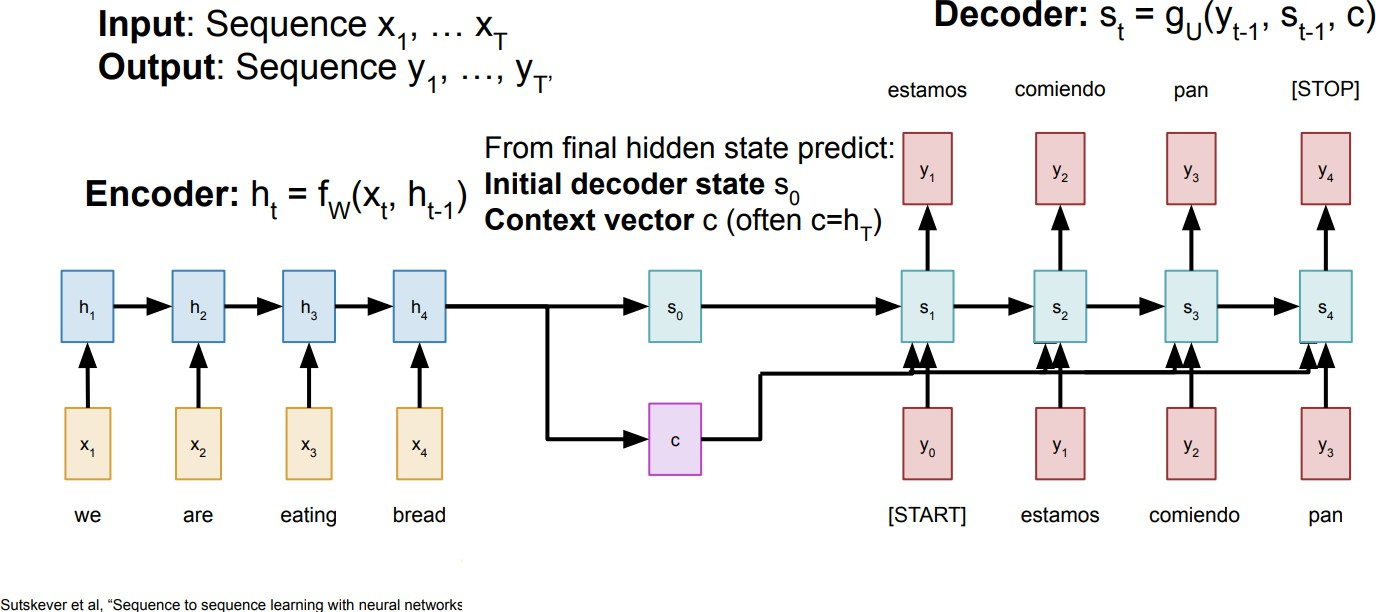
\includegraphics[width=1.05\textwidth,keepaspectratio]{images/rnn/slide_10_1_img.jpg}
    \end{figure}

    \framebreak

    \begin{figure}
        \centering
        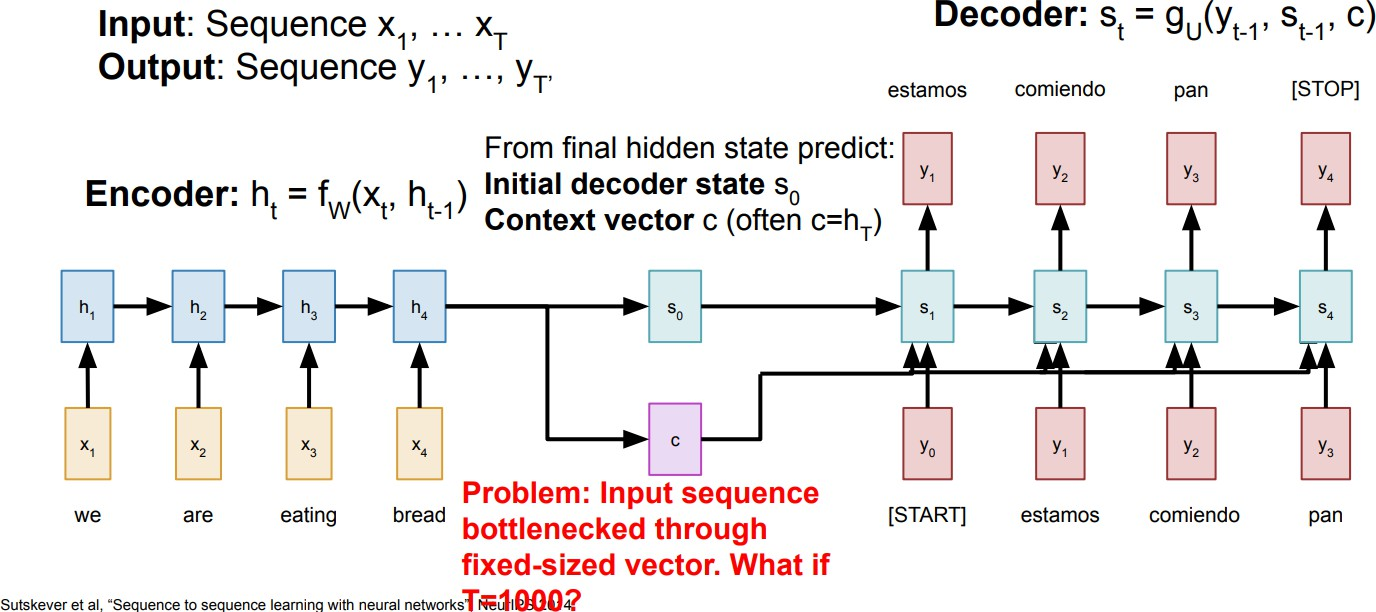
\includegraphics[width=1.05\textwidth,keepaspectratio]{images/rnn/slide_11_1_img.jpg}
    \end{figure}

    \framebreak

    \begin{figure}
        \centering
        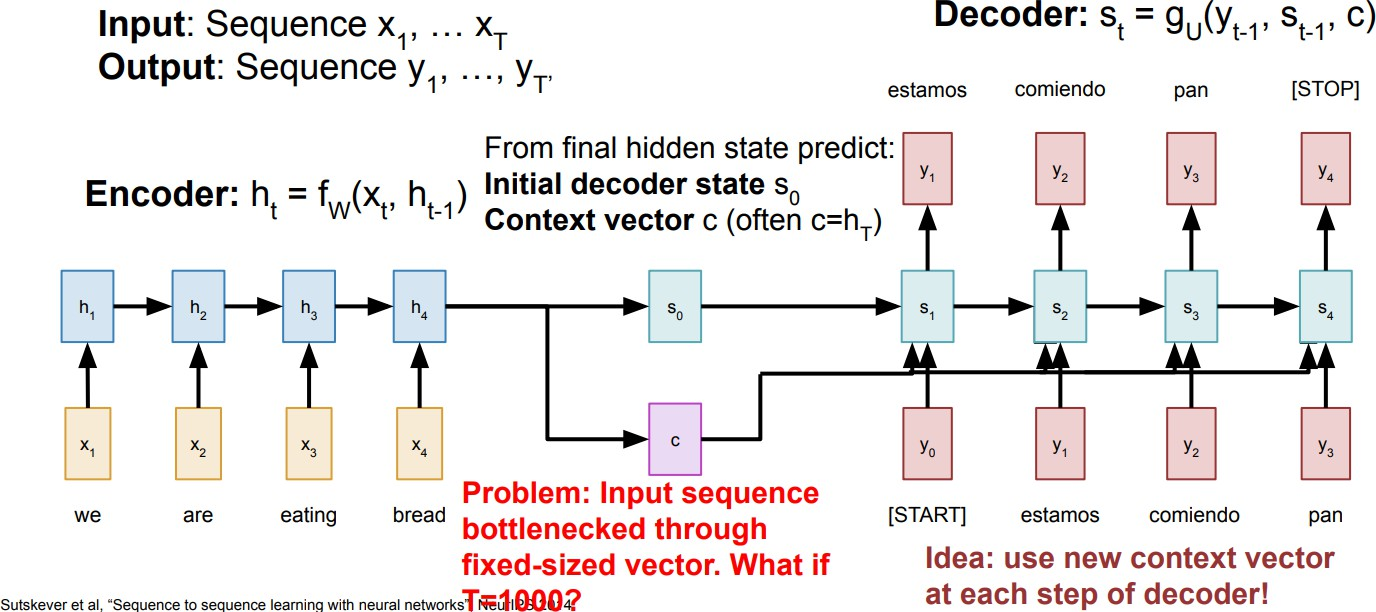
\includegraphics[width=1.05\textwidth,keepaspectratio]{images/rnn/slide_12_1_img.jpg}
    \end{figure}
\end{frame}


\begin{frame}[allowframebreaks]{Sequence to Sequence based on sentence length}
    \begin{figure}
        \centering
        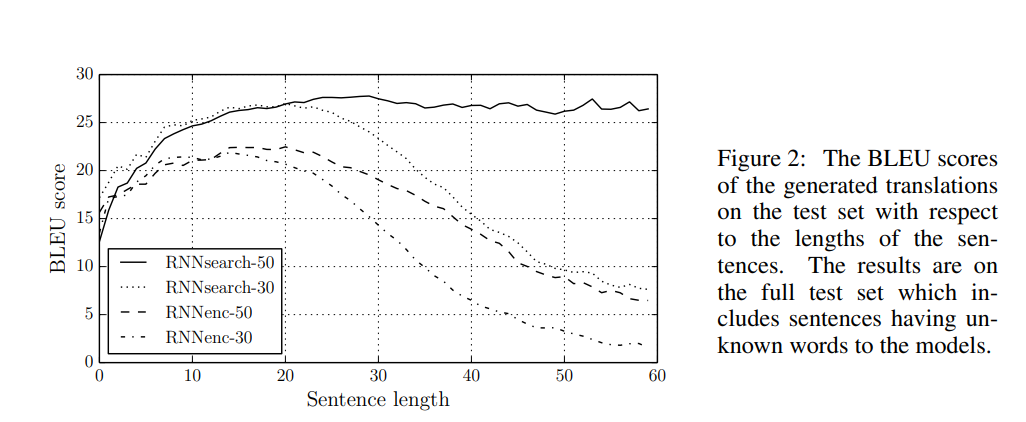
\includegraphics[width=1.05\textwidth,keepaspectratio]{images/rnn/slide_13_1_img.png}
    \end{figure}
\end{frame}


\begin{frame}[allowframebreaks]{Sequence to Sequence Calculating H states}
    \begin{figure}
        \centering
        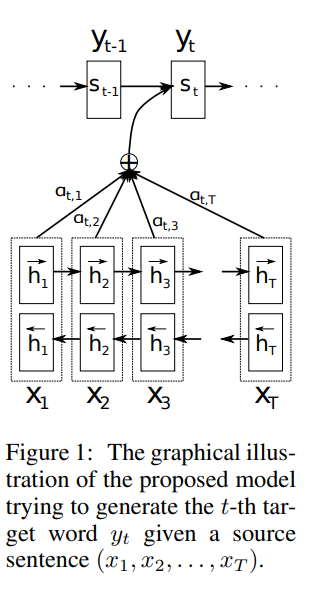
\includegraphics[height=0.9\textheight,keepaspectratio]{images/rnn/slide_14_1_img.png}
    \end{figure}
\end{frame}


\begin{frame}[allowframebreaks]{Sequence to Sequence with RNNs and Attention}
    \begin{figure}
        \flushleft
        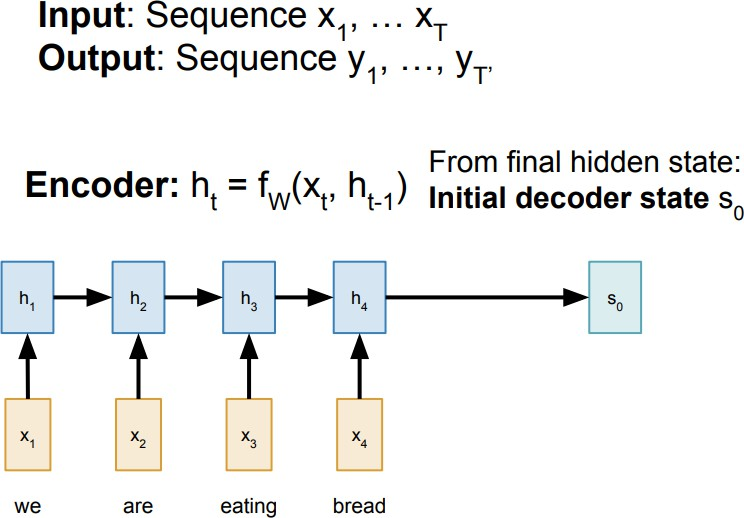
\includegraphics[width=0.6\textwidth,keepaspectratio]{images/rnn/slide_15_1_img.jpg}
    \end{figure}

    \framebreak

    \begin{figure}
        \centering
        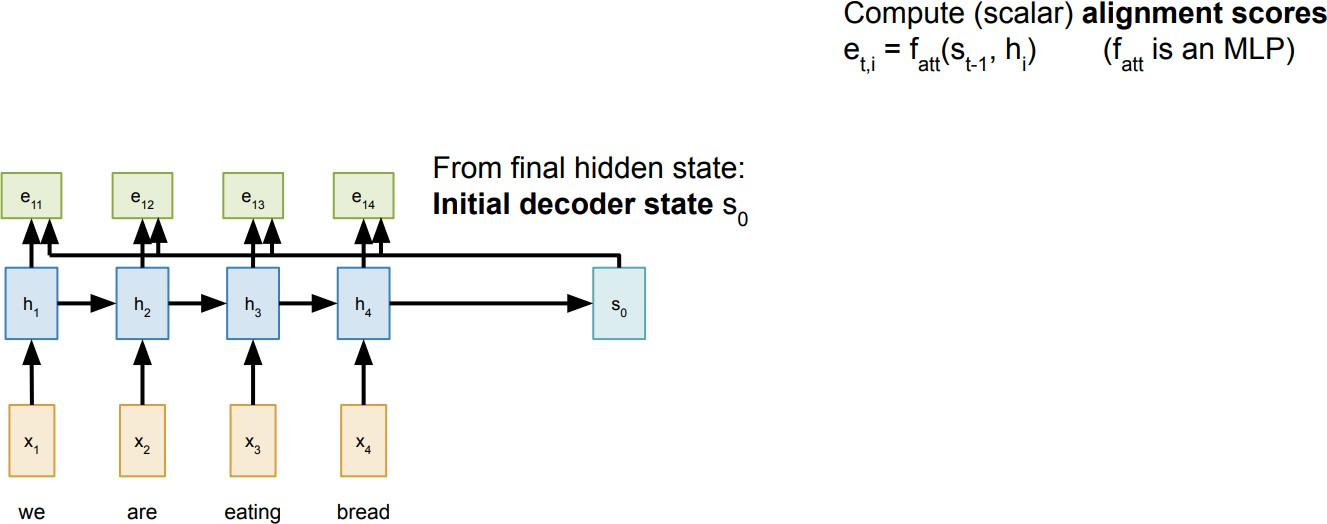
\includegraphics[width=1\textwidth,keepaspectratio]{images/rnn/slide_16_1_img.jpg}
    \end{figure}

    \framebreak

    \begin{figure}
        \centering
        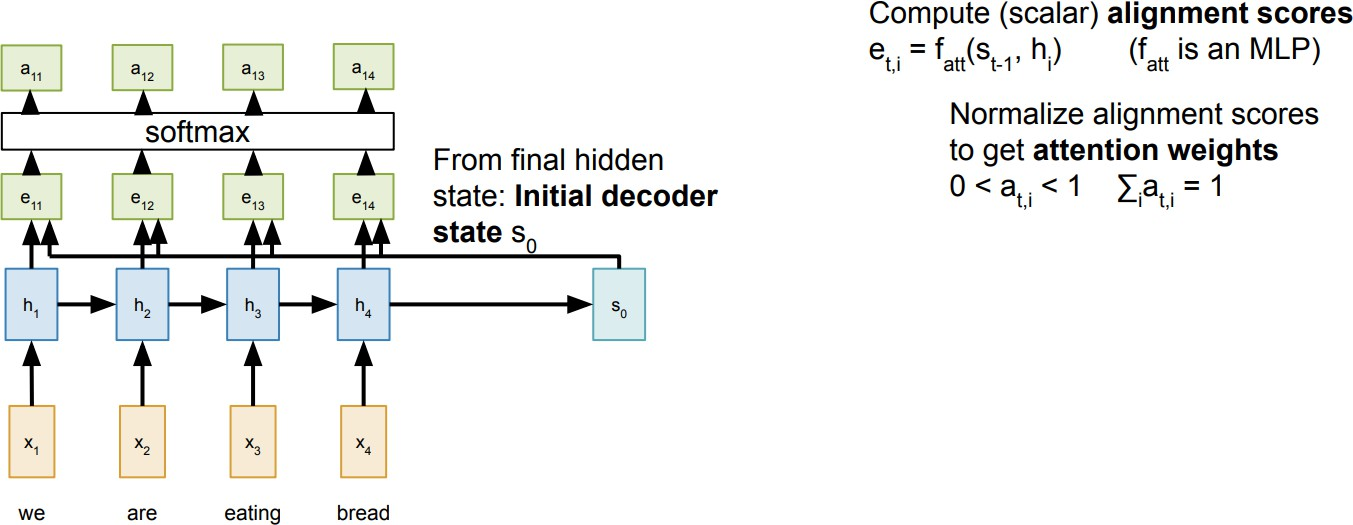
\includegraphics[width=1\textwidth,keepaspectratio]{images/rnn/slide_17_1_img.jpg}
    \end{figure}

    \framebreak

    \begin{figure}
        \centering
        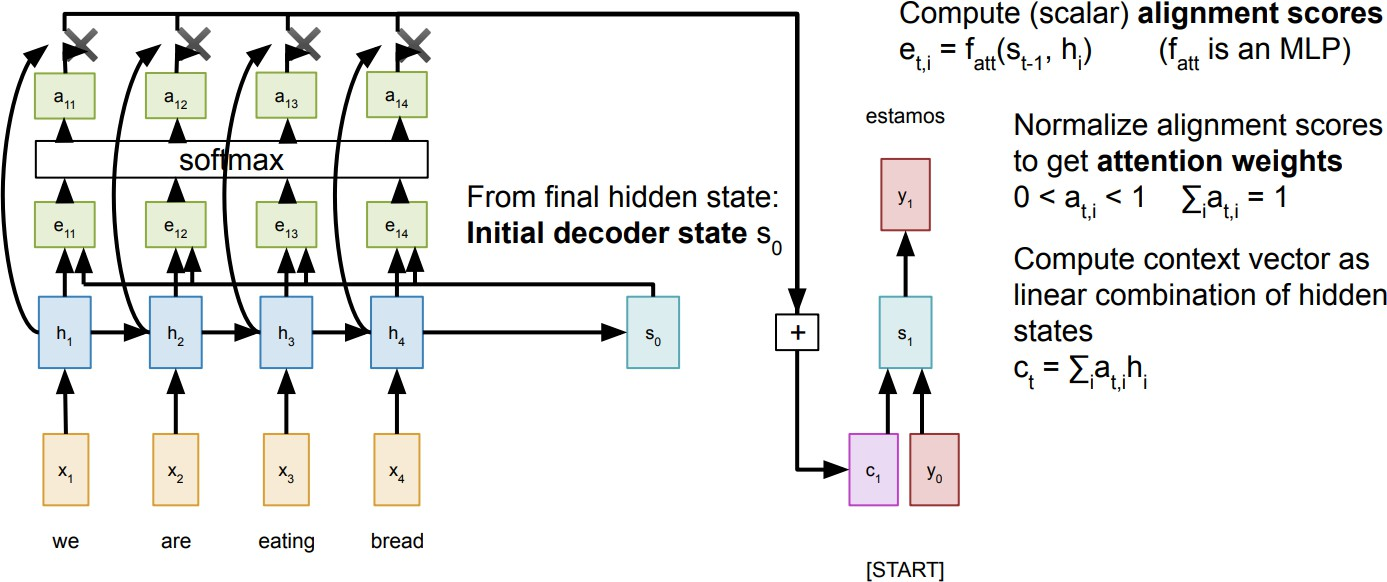
\includegraphics[width=1\textwidth,keepaspectratio]{images/rnn/slide_18_1_img.jpg}
    \end{figure}

    \framebreak

    \begin{figure}
        \centering
        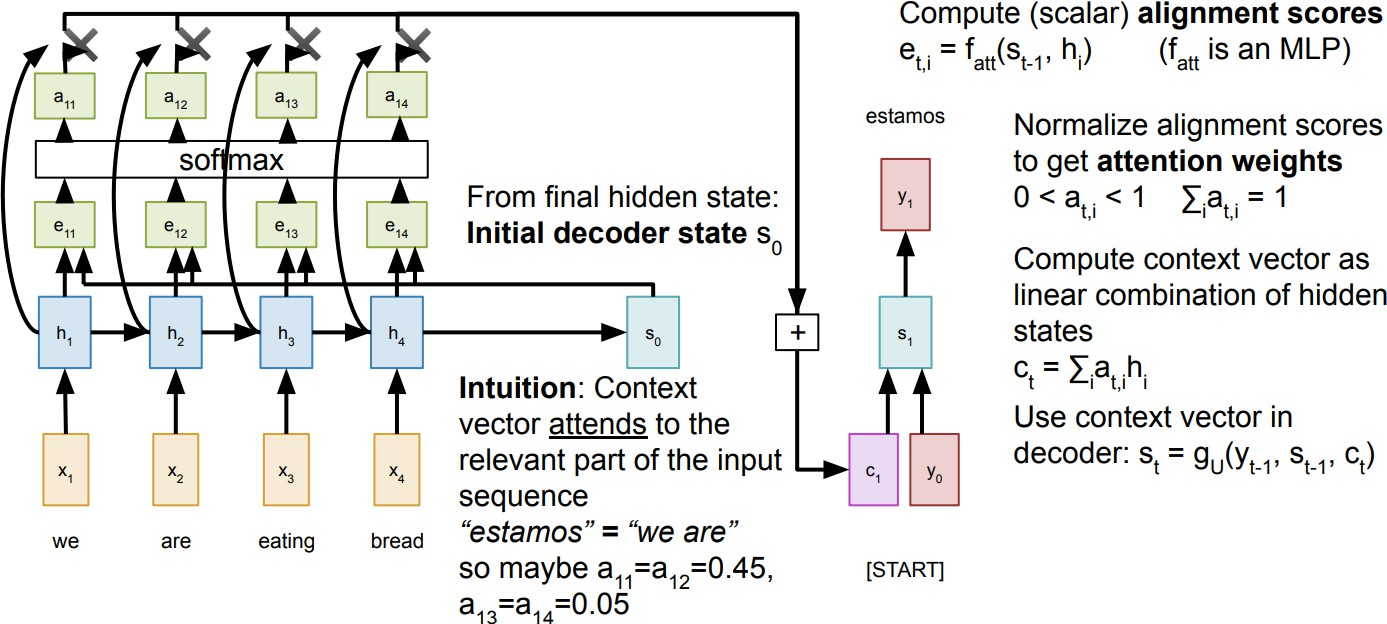
\includegraphics[width=1\textwidth,keepaspectratio]{images/rnn/slide_19_1_img.jpg}
    \end{figure}

    \framebreak

    \begin{figure}
        \centering
        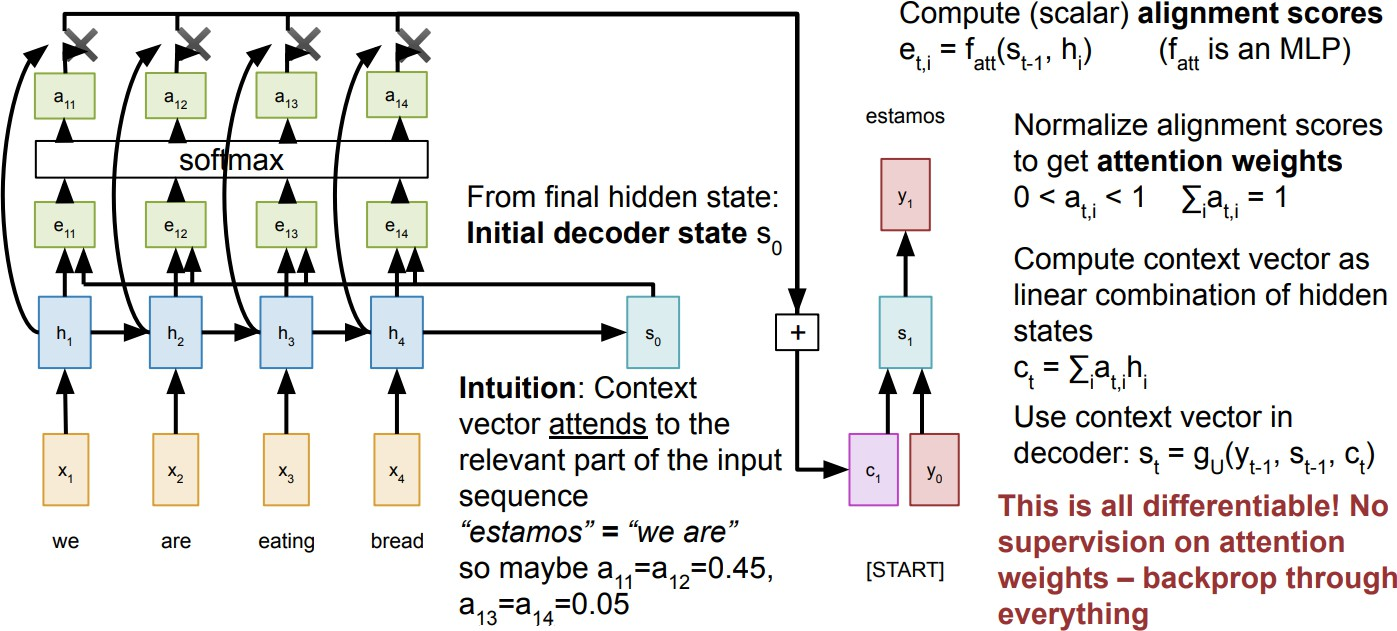
\includegraphics[width=1\textwidth,keepaspectratio]{images/rnn/slide_20_1_img.jpg}
    \end{figure}

    \framebreak

    \begin{figure}
        \centering
        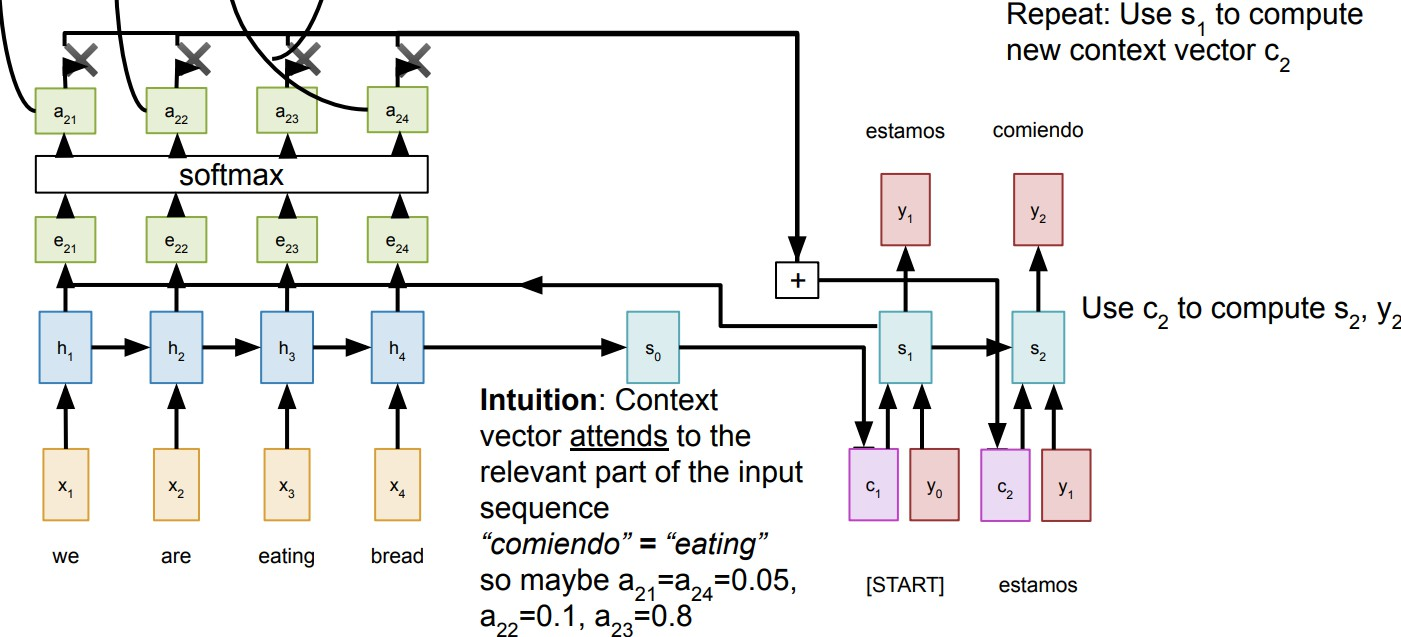
\includegraphics[width=1\textwidth,keepaspectratio]{images/rnn/slide_21_1_img.jpg}
    \end{figure}

    \framebreak
    \begin{itemize}
        \item \textbf{Dynamic Context Vector at Each Decoder Timestep:}
        \begin{itemize}
            \setlength{\itemsep}{-0.5em}
            \item Instead of using a single, fixed context vector for all decoding steps, a different context vector is computed at each timestep of the decoder.
            \item This approach prevents the input sequence from being bottlenecked through a single vector, allowing richer information flow.
            \item At every decoding step, the context vector dynamically attends to different parts of the input sequence, enabling the decoder to focus on the most relevant information for generating each output token.
        \end{itemize}
    \end{itemize}
    \begin{figure}
        \centering
        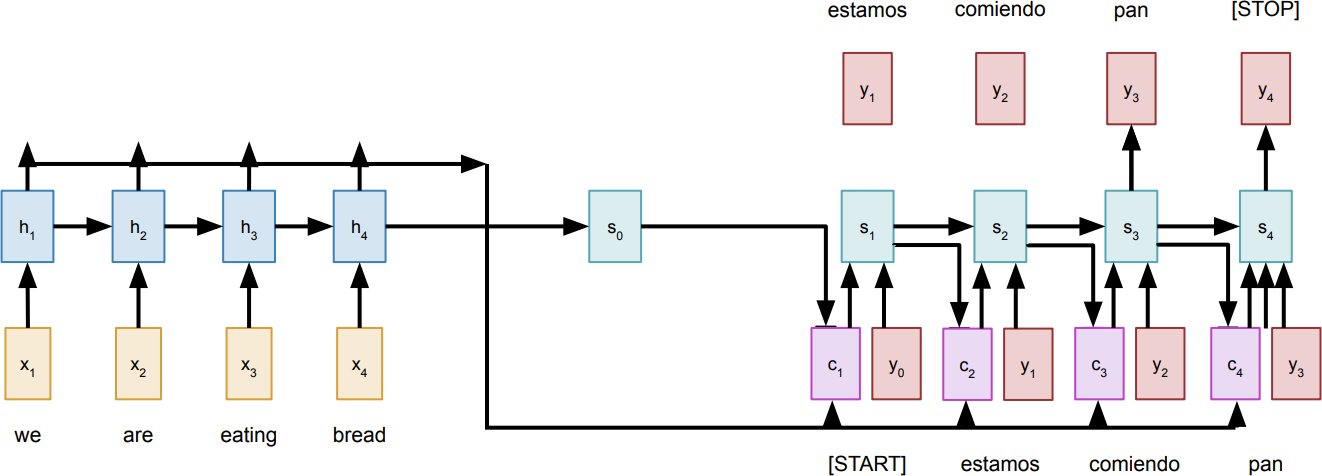
\includegraphics[width=1\textwidth,keepaspectratio]{images/rnn/slide_22_1_img.png}
    \end{figure}

    \framebreak

    \begin{figure}
        \centering
        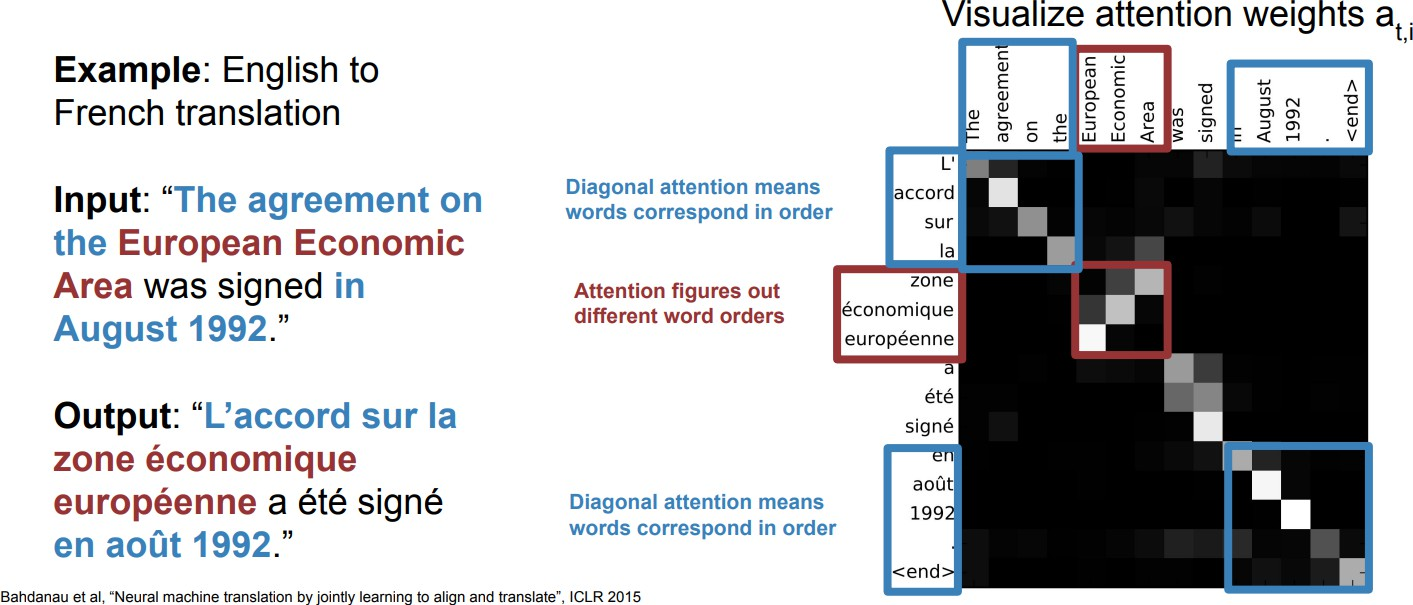
\includegraphics[width=1\textwidth,keepaspectratio]{images/rnn/slide_23_1_img.jpg}
    \end{figure}

    \framebreak

    \begin{figure}
        \flushleft
        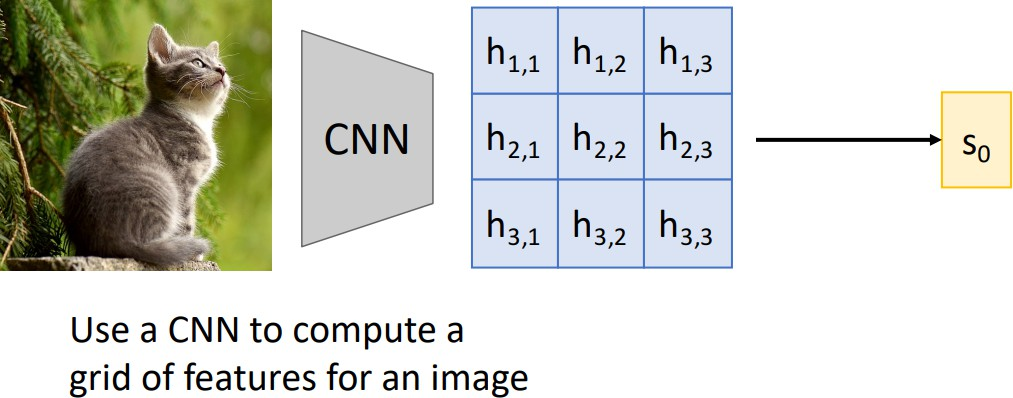
\includegraphics[width=0.6\textwidth,keepaspectratio]{images/rnn/slide_24_1_img.jpg}
    \end{figure}

    \framebreak

    \begin{figure}
        \flushleft
        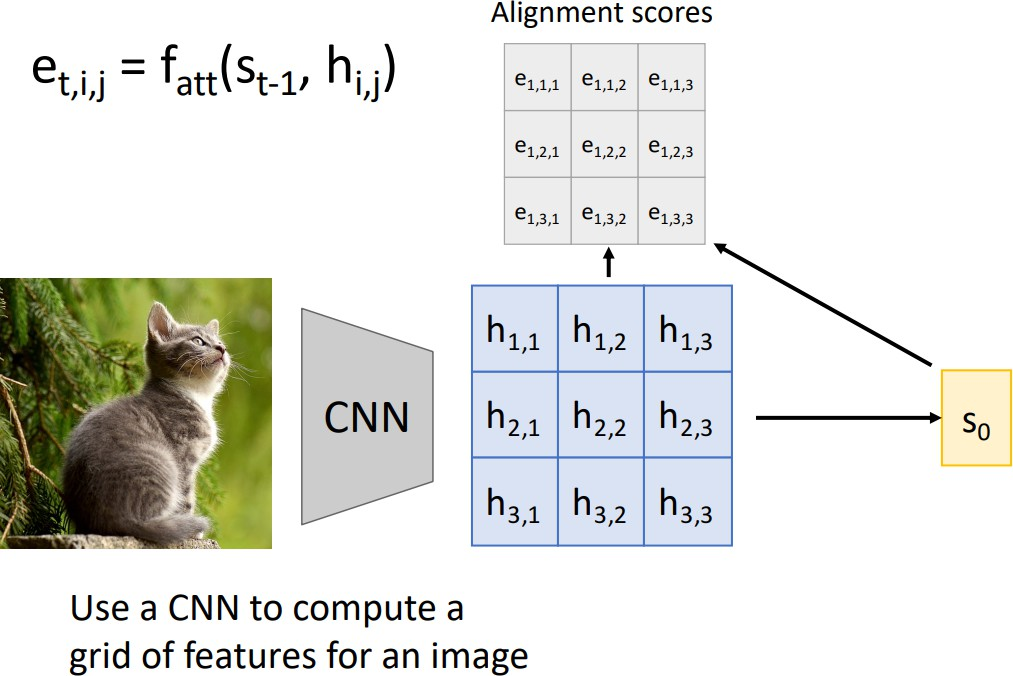
\includegraphics[width=0.6\textwidth,keepaspectratio]{images/rnn/slide_25_1_img.jpg}
    \end{figure}

    \framebreak

    \begin{figure}
        \flushleft
        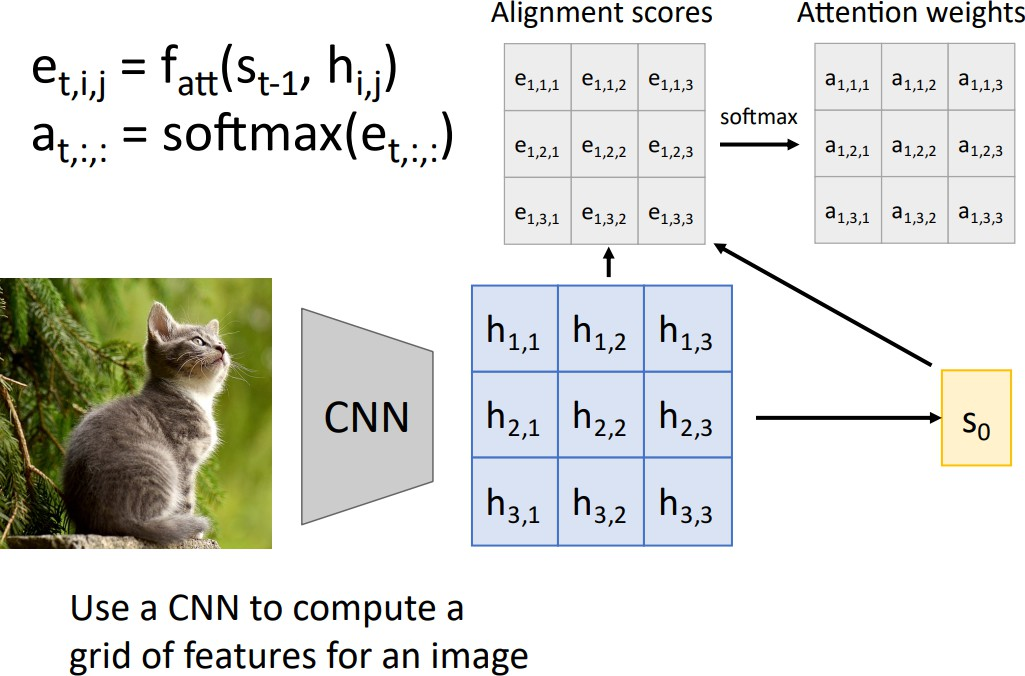
\includegraphics[width=0.6\textwidth,keepaspectratio]{images/rnn/slide_26_1_img.jpg}
    \end{figure}

    \framebreak

    \begin{figure}
        \flushleft
        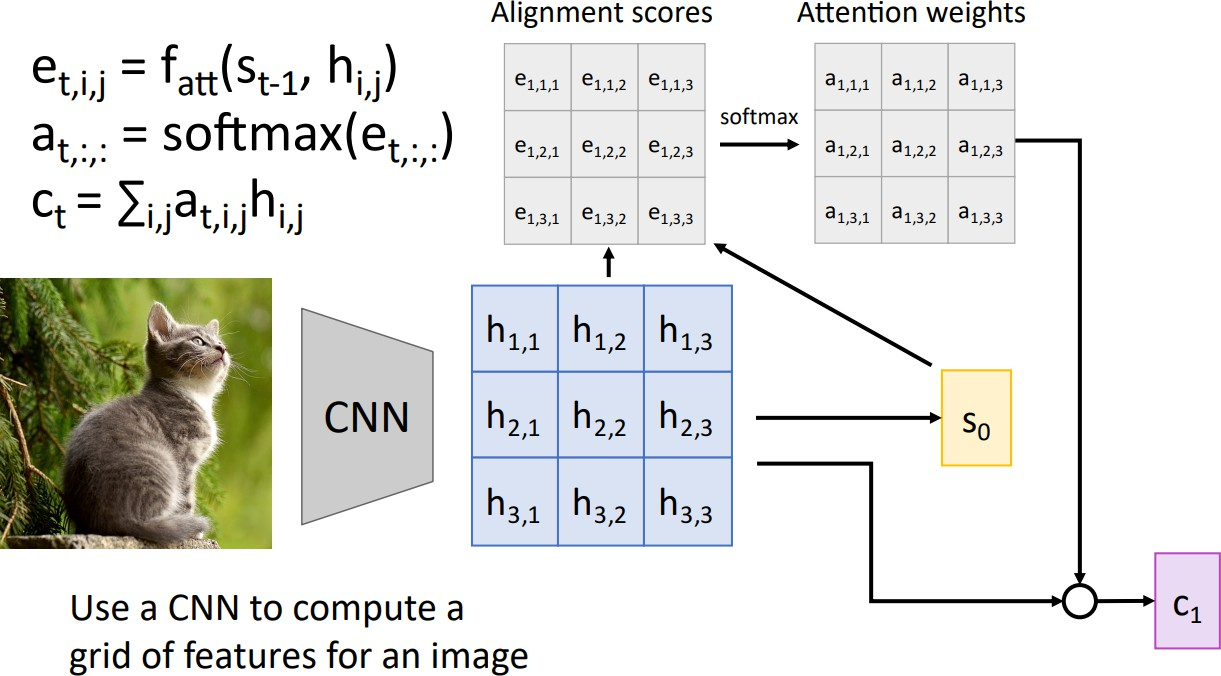
\includegraphics[width=0.7\textwidth,keepaspectratio]{images/rnn/slide_27_1_img.jpg}
    \end{figure}

    \framebreak

    \begin{figure}
        \flushleft
        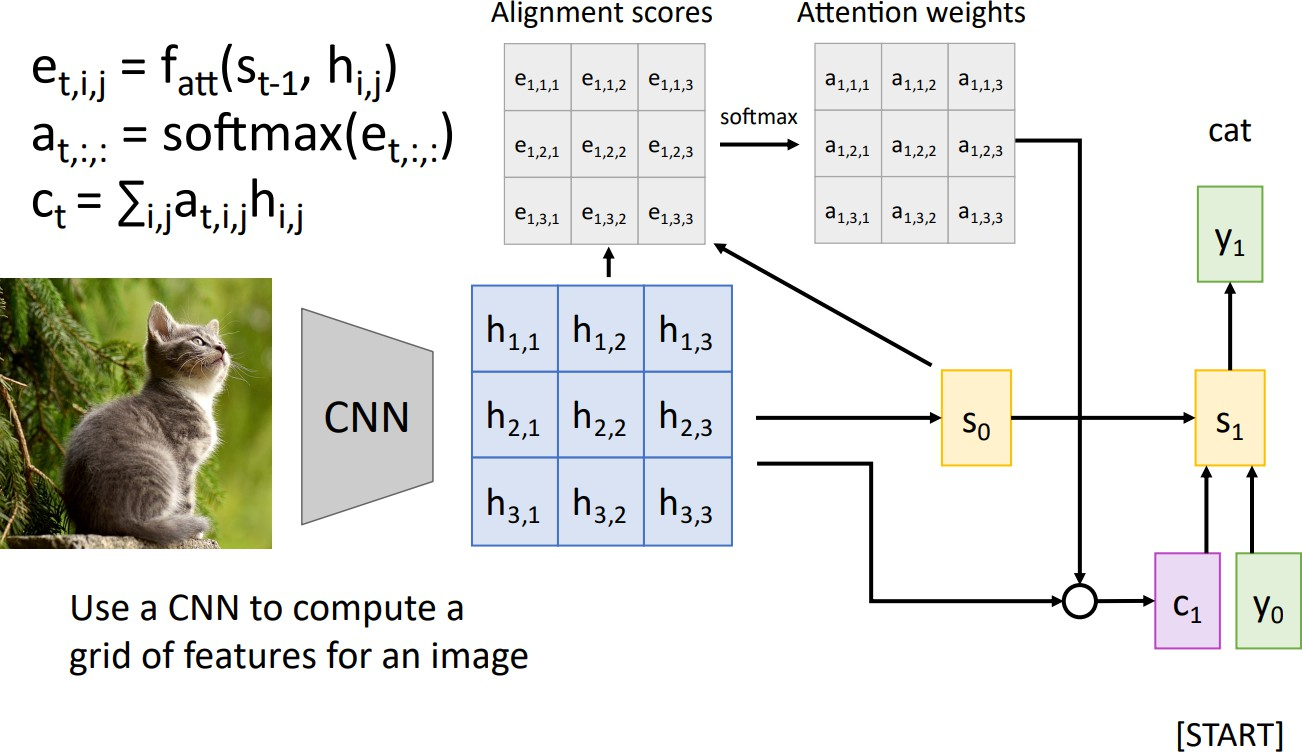
\includegraphics[width=0.75\textwidth,keepaspectratio]{images/rnn/slide_28_1_img.jpg}
    \end{figure}

    \framebreak

    \begin{figure}
        \flushleft
        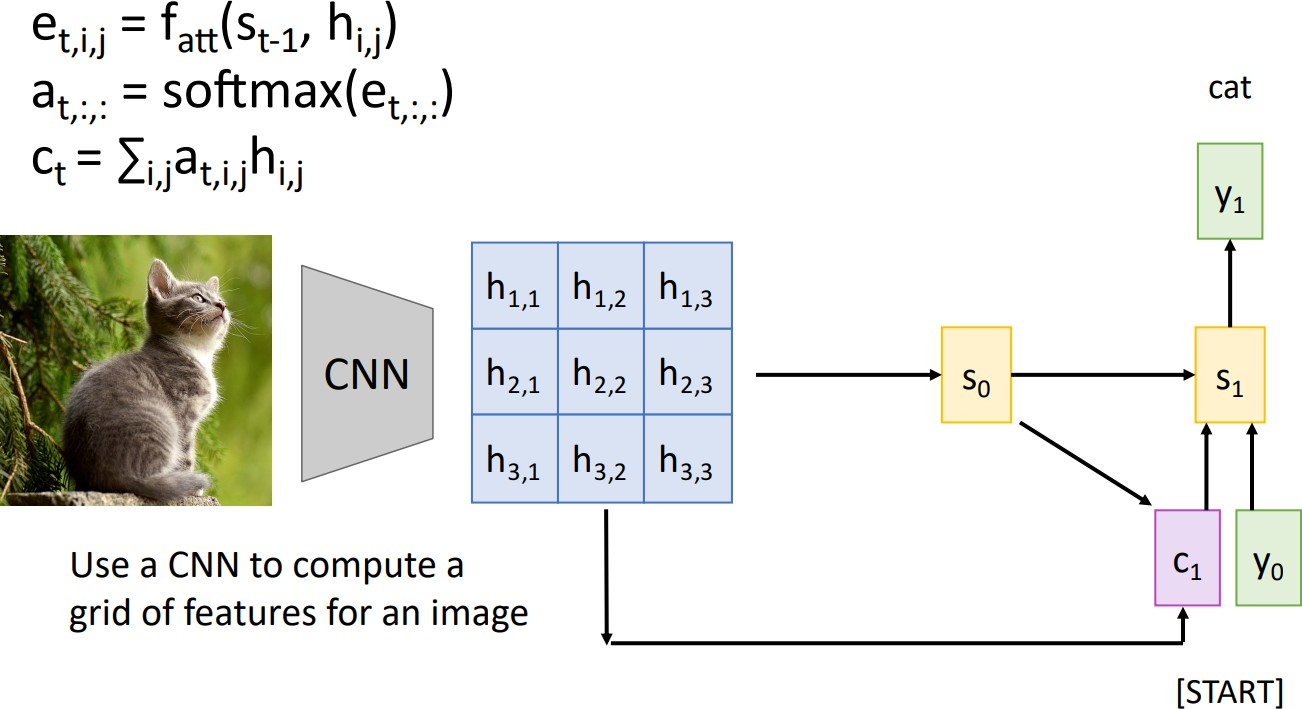
\includegraphics[width=0.75\textwidth,keepaspectratio]{images/rnn/slide_29_1_img.jpg}
    \end{figure}

    \framebreak

    \begin{figure}
        \flushleft
        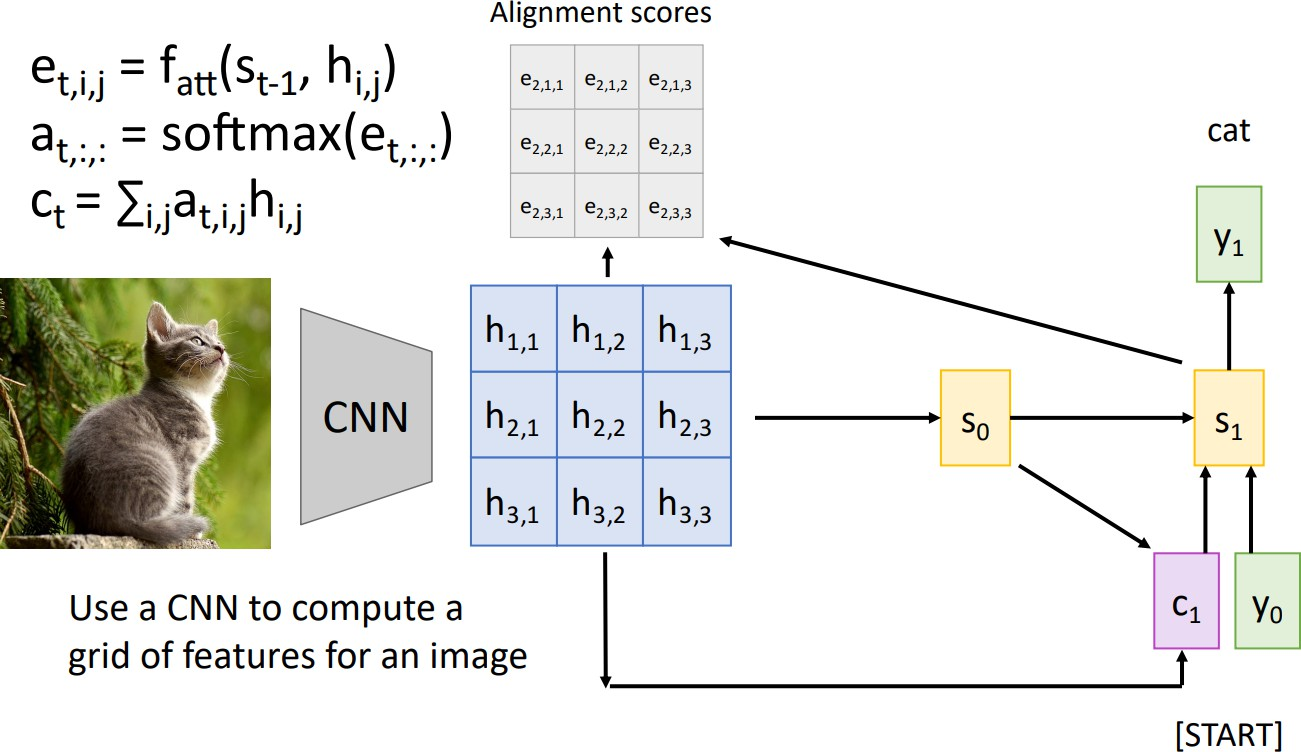
\includegraphics[width=0.75\textwidth,keepaspectratio]{images/rnn/slide_30_1_img.jpg}
    \end{figure}

    \framebreak

    \begin{figure}
        \flushleft
        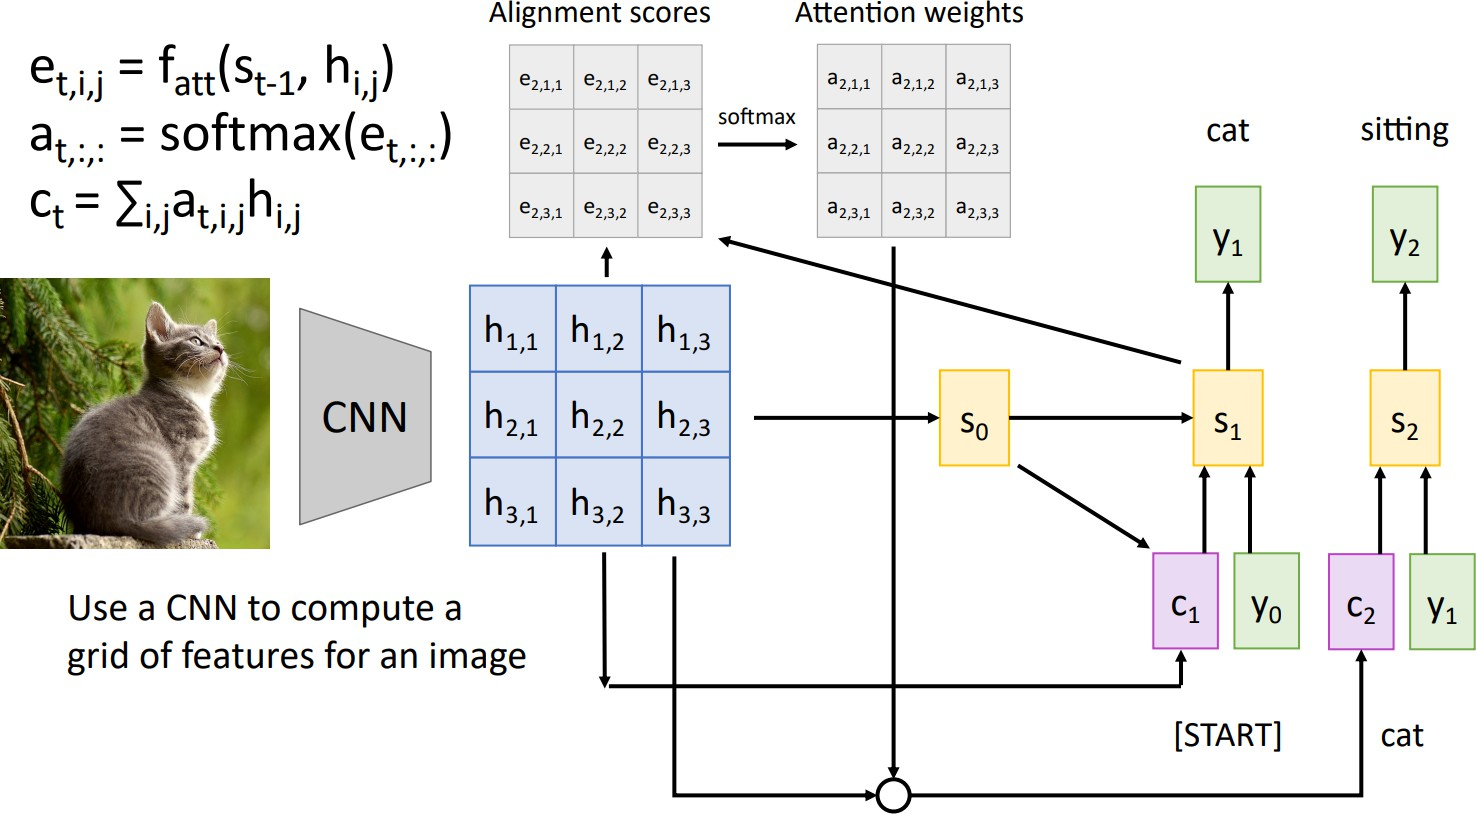
\includegraphics[width=0.85\textwidth,keepaspectratio]{images/rnn/slide_31_1_img.jpg}
    \end{figure}

    \framebreak

    \begin{figure}
        \centering
        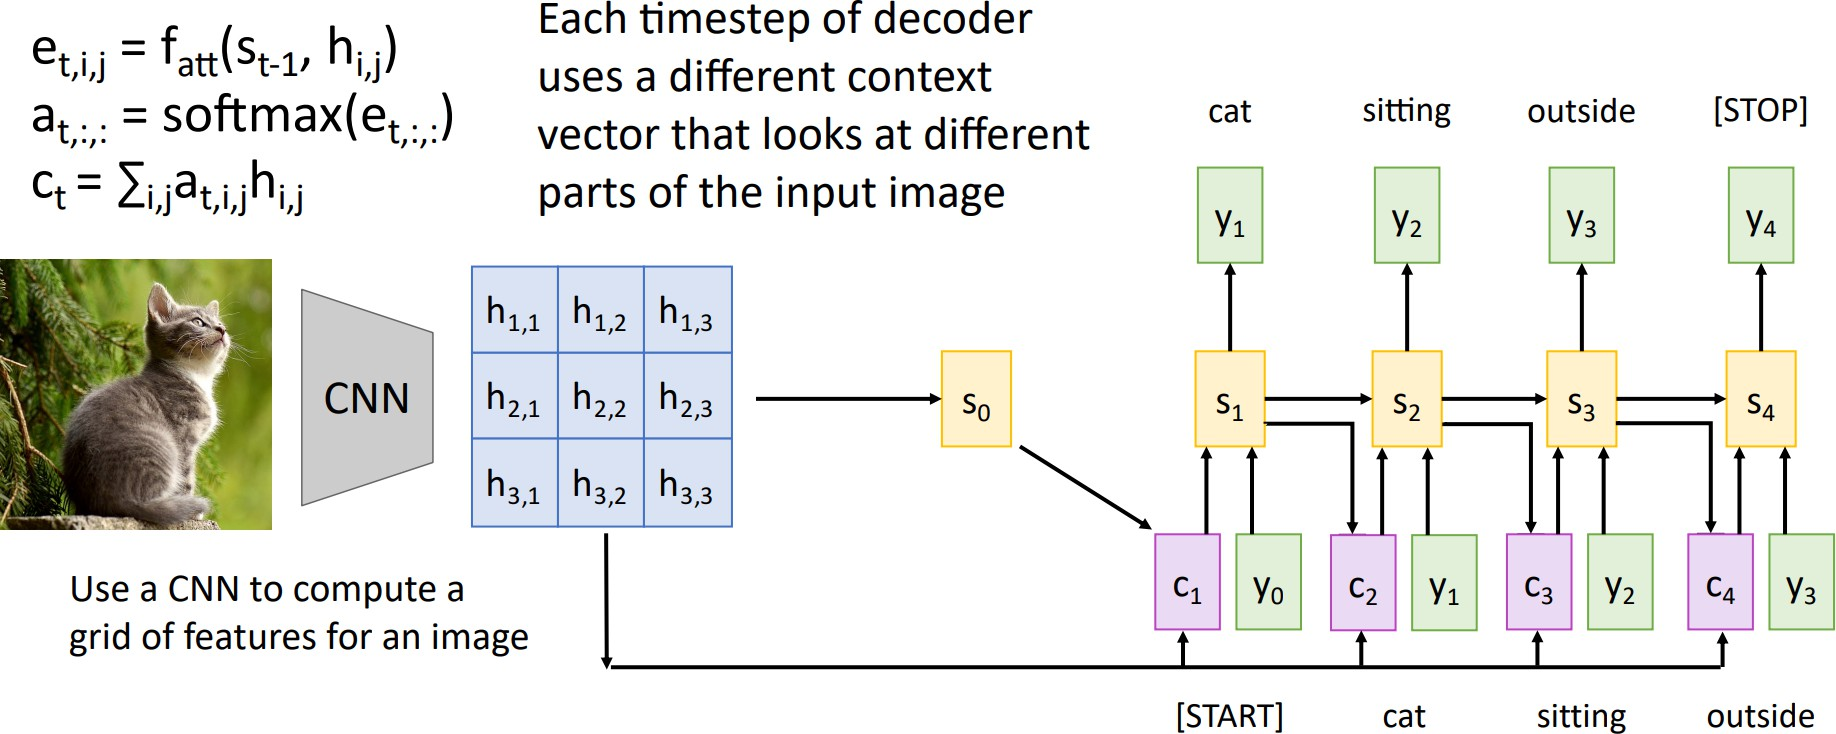
\includegraphics[width=1\textwidth,keepaspectratio]{images/rnn/slide_32_1_img.jpg}
    \end{figure}

    \framebreak

    \begin{figure}
        \centering
        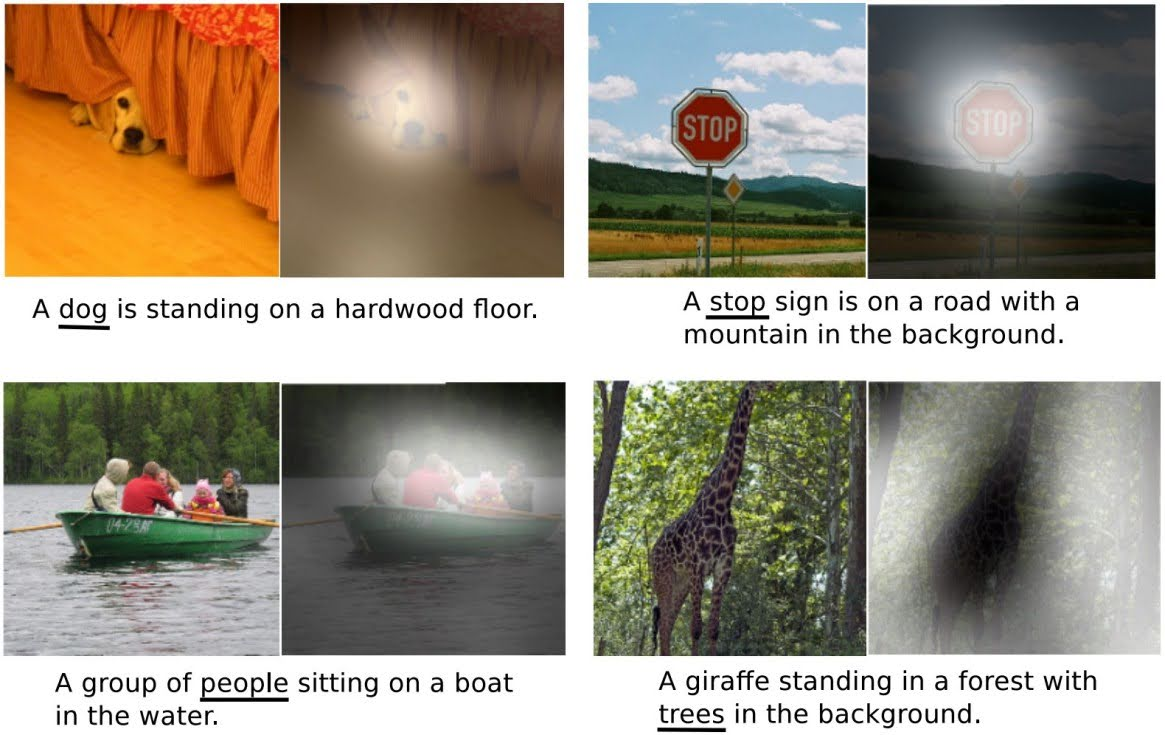
\includegraphics[width=1\textwidth,keepaspectratio]{images/rnn/slide_33_1_img.png}
    \end{figure}
    \footnote{Xu et al, “Show, AKend, and Tell: Neural Image CapAon GeneraAon with Visual AKenAon”, ICML 2015}
\end{frame}


\begin{frame}[allowframebreaks]{Attention we just saw in image captioning}
    \begin{figure}
        \centering
        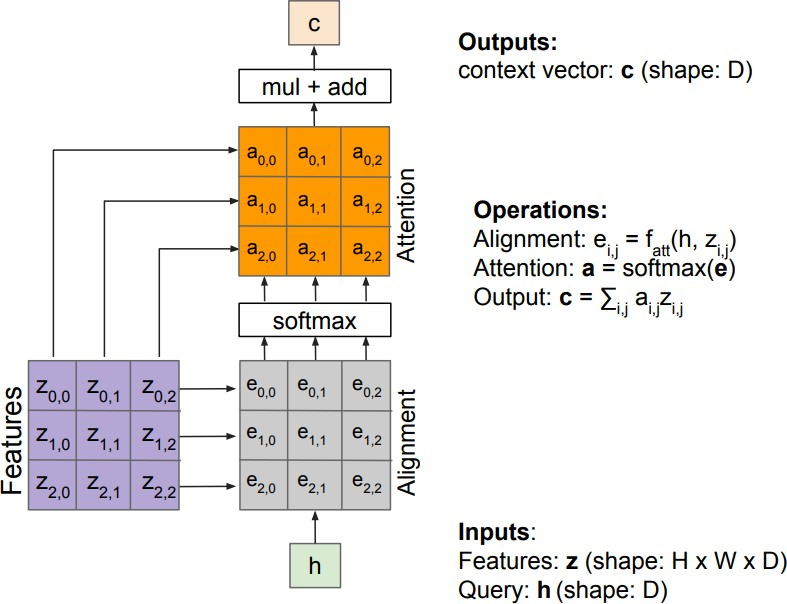
\includegraphics[width=0.9\textwidth,height=0.9\textheight,keepaspectratio]{images/rnn/slide_34_1_img.jpg}
    \end{figure}
\end{frame}